\documentclass[a4paper,12pt]{article}

\usepackage{float}


\usepackage[utf8]{inputenc}
\usepackage[dvips]{graphicx}
%\usepackage{a4wide}
\usepackage{epsfig}
\usepackage{fancybox}
\usepackage{verbatim}
\usepackage{array}
\usepackage{latexsym}
\usepackage{alltt}
\usepackage{amssymb}
\usepackage{amsmath,amsthm}
\usepackage{bm}
\usepackage{wasysym}

%\usepackage{fullpage}
%\usepackage{hyperref}
\usepackage{listings}
\usepackage{color}
\usepackage{algorithm}
\usepackage{algpseudocode}
\usepackage[hmargin=2cm,vmargin=3.0cm]{geometry}
%\topmargin=0cm
%\topmargin=-1.8cm
%\addtolength{\textheight}{6.5cm}
%\addtolength{\textwidth}{2.0cm}
%\setlength{\leftmargin}{-3cm}
%\setlength{\oddsidemargin}{0.0cm}
%\setlength{\evensidemargin}{0.0cm}

%misc libraries goes here
\usepackage{tikz}
\usepackage{tikz-qtree}
\usetikzlibrary{automata,positioning}

\usepackage{multicol}
\usepackage{enumitem}

\usepackage[most]{tcolorbox}

\usepackage[colorlinks=true,urlcolor=black,linkcolor=black]{hyperref}
\hbadness=10000

\lstdefinestyle{customtex}{
    %backgroundcolor=\color{lbcolor},
    tabsize=2,
    language=TeX,
    numbers=none,
    basicstyle=\footnotesize\ttfamily,
    numberstyle=\footnotesize,
    aboveskip={0.0\baselineskip},
    belowskip={0.0\baselineskip},
    %
    columns=flexible,
    keepspaces=true,
    fontadjust=true,
    upquote=true,
    %
    breaklines=true,
    prebreak=\raisebox{0ex}[0ex][0ex]{\ensuremath{\hookleftarrow}},
    frame=single,
    showtabs=false,
    showspaces=false,
    showstringspaces=false,
    %
    %identifierstyle=\color[rgb]{0,0.2,0.8},
    identifierstyle=\color[rgb]{0,0,0.5},
    %identifierstyle=\color[rgb]{0.133,0.545,0.133},
    %keywordstyle=\color[rgb]{0.8,0,0},
    %keywordstyle=\color[rgb]{0.133,0.545,0.133},
    keywordstyle=\color[rgb]{0,0,0.5},
    %commentstyle=\color[rgb]{0.133,0.545,0.133},
    commentstyle=\color[rgb]{0.545,0.545,0.545},
    %stringstyle=\color[rgb]{0.827,0.627,0.133},
    stringstyle=\color[rgb]{0.133,0.545,0.133},
    %
    literate={â}{{\^{a}}}1 {Â}{{\^{A}}}1 {ç}{{\c{c}}}1 {Ç}{{\c{C}}}1 {ğ}{{\u{g}}}1 {Ğ}{{\u{G}}}1 {ı}{{\i}}1 {İ}{{\.{I}}}1   {ö}{{\"o}}1 {Ö}{{\"O}}1 {ş}{{\c{s}}}1 {Ş}{{\c{S}}}1 {ü}{{\"u}}1 {Ü}{{\"U}}1 {~}{$\sim$}{1}
}

\lstdefinestyle{output}{
    %backgroundcolor=\color{lbcolor},
    tabsize=2,
    numbers=none,
    basicstyle=\footnotesize\ttfamily,
    numberstyle=\footnotesize,
    aboveskip={0.0\baselineskip},
    belowskip={0.0\baselineskip},
    %
    columns=flexible,
    keepspaces=true,
    fontadjust=true,
    upquote=true,
    %
    breaklines=true,
    prebreak=\raisebox{0ex}[0ex][0ex]{\ensuremath{\hookleftarrow}},
    frame=single,
    showtabs=false,
    showspaces=false,
    showstringspaces=false,
    %
    %identifierstyle=\color[rgb]{0.44,0.12,0.1},
    identifierstyle=\color[rgb]{0,0,0},
    keywordstyle=\color[rgb]{0,0,0},
    commentstyle=\color[rgb]{0,0,0},
    stringstyle=\color[rgb]{0,0,0},
    %
    literate={â}{{\^{a}}}1 {Â}{{\^{A}}}1 {ç}{{\c{c}}}1 {Ç}{{\c{C}}}1 {ğ}{{\u{g}}}1 {Ğ}{{\u{G}}}1 {ı}{{\i}}1 {İ}{{\.{I}}}1   {ö}{{\"o}}1 {Ö}{{\"O}}1 {ş}{{\c{s}}}1 {Ş}{{\c{S}}}1 {ü}{{\"u}}1 {Ü}{{\"U}}1
}

\lstset{style=customtex}


\tikzset{%
    terminal/.style={draw, rectangle,
    				 align=center, 
					 minimum height=1cm, 
					 minimum width=2cm,
					 fill=black!10,
					 anchor=mid},
    nonterminal/.style={draw, rectangle,
    					align=left,
					    minimum height=1cm, 
						minimum width=2cm, 
						anchor=mid},% and so on
}

%% Style for terminals
%\tikzstyle{terminal}=[draw, rectangle, 
%					  minimum height=1cm, 
%					  minimum width=2cm, 
%					  fill=black!20,
%					  anchor=south west]
%% Style for nonterminals
%\tikzstyle{nonterminal}=[draw, rectangle, 
%						 minimum height=1 cm, 
%						 minimum width=2 cm, 
%						 anchor=north east]


\newcommand{\HRule}{\rule{\linewidth}{1mm}}
\newcommand{\kutu}[2]{\framebox[#1mm]{\rule[-2mm]{0mm}{#2mm}}}
\newcommand{\gap}{ \\[1mm] }

\newcommand{\Q}{\raisebox{1.7pt}{$\scriptstyle\bigcirc$}}
\newcommand{\minus}{\scalebox{0.35}[1.0]{$-$}}

\setlength{\fboxsep}{10pt}

\tcbsetforeverylayer{enhanced jigsaw, breakable, arc=0mm, boxrule=1pt, boxsep=5pt, after=\vspace{1em}, colback=white, colframe=black}

\newcolumntype{P}[1]{>{\centering\arraybackslash}p{#1}}

\setlength\parindent{0pt}

%\renewcommand\arraystretch{1.2}

\newenvironment{Tab}[1]
  {\def\arraystretch{1}\tabular{#1}}
  {\endtabular}

%%%%%%%%%%%%%%%%%%%%%%%%%%%%%%%%%%%%%%%%%%%%%%%%%%%%%%%%%%%%%%%%%%%%%%%%%%%%%%%%%%%%%%

\title{Formal Languages and Abstract Machines \\ Take Home Exam 2}
\author{Yasin Fatih ALPUL \\ 2098739} % write your name and id
\date{} % do not write any date

%%%%%%%%%%%%%%%%%%%%%%%%%%%%%%%%%%%%%%%%%%%%%%%%%%%%%%%%%%%%%%%%%%%%%%%%%%%%%%%%%%%%%%

\begin{document}
\HRule\\
Middle East Technical University \hfill Department of Computer Engineering
{\let\newpage\relax\maketitle}
\HRule\\
\vspace{1cm}

%%%%%%%%%%%%%%%%%%%%%%%%%%%%%%%%%%%%%%%%%%%%%%%%%%%%%%%%%%%%%%%%%%%%%%%%%%%%%%%%%%%%%%

% Write your answers below the section tags
\section{Context-Free Grammars \hfill \normalfont{(10 pts)}}

\paragraph{a)} Give the rules of the Context-Free Grammars to recognize strings in the given languages where $\Sigma=\{a,b\}$ and $S$ is the start symbol. \\  

$L(G)=\{w \mid \;  w \in \Sigma^*;\; |w| \geq 3;\; $  \hfill \small{(2/10 pts)} \\
\hspace*{22mm} the first and the second from the last symbols of $w$ are the same$\}$ \\

\begin{tcolorbox}
\begin{align*}
    S & \rightarrow aXaY~|~bXbY\\
    Y & \rightarrow a~|~b\\
    X & \rightarrow aX~|~bX~|~e\\
\end{align*}
\end{tcolorbox}


$L(G)=\{w \mid \;  w \in \Sigma^*;\; $ the length of w is odd$\}$ \hfill \small{(2/10 pts)} \\

\begin{tcolorbox}
\begin{align*}
    S &\rightarrow aX | bX\\
    X &\rightarrow aaX | abX | baX | bbX | e
\end{align*}
\end{tcolorbox}


$L(G)=\{w \mid \;  w \in \Sigma^*;\; n(w,a)=2\cdot n(w,b)\}$ where $n(w,x)$ is the number of $x$ symbols in $w$ \hfill \small{(3/10 pts)} \\
\begin{tcolorbox}
\[
    S  \rightarrow SaSaSbS|SaSbSaS|SbSaSaS|e
\]
\end{tcolorbox}

\paragraph{b)} Find the set of strings recognized by the CFG rules given below:         \hfill \small{(3/10 pts)} \\


$S \to X \mid Y$ \\
$X \to aXb \mid A \mid B$ \\
$A \to aA \mid a$ \\
$B \to Bb \mid b$ \\
$Y \to CbaC$ \\
$C \to CC \mid a \mid b \mid \varepsilon$  \\

\begin{tcolorbox}
The set of strings recognized by the rules is the union of the following two sets:\\
\[
\{a^nb^m : n,m > 0\}
\]
\[
\{w : w \text{ contains }ba\text{ as a substring and } |w|\text{ is even}\}
\]
\end{tcolorbox}


\newpage
\section{Parse Trees and Derivations \hfill \normalfont{(20 pts)}}
Given the CFG below, provide parse trees for given sentences in \textbf{a} and \textbf{b}.\\

\begin{lstlisting}[style=output,mathescape=true]
S   $\to$ NP VP
VP  $\to$ V NP | V NP PP
PP  $\to$ P NP
NP  $\to$ N | D N | NP PP
V   $\to$ wrote | built | constructed
D   $\to$ a | an | the | my
N   $\to$ John | Mary | Jane | man | book | automata | pen | class
P   $\to$ in | on | by | with
\end{lstlisting}

\paragraph{a)} Jane constructed automata with a pen \hfill \small{(4/20 pts)} \\

\begin{tcolorbox}
\Tree [.S [.NP [.N Jane ] ] [.VP [.V constructed ] [.NP [.N automata ] ] [.PP [.P with ] [.NP [.D a ] [.N pen ] ] ] ] ]
\Tree [.S [.NP [.N Jane ] ] [.VP [.V constructed ] [.NP [.NP [.N automata ] ] [.PP [.P with ] [.NP [.D a ] [.N pen ] ] ] ] ] ]
\end{tcolorbox}

\paragraph{b)} my book in the man built a Jane by a pen \hfill \small{(4/20 pts)} \\

\begin{tcolorbox}
\Tree [.S [.NP [.NP [.D my ] [.N book ] ] [.PP [.P in ] [.NP [.D the ] [.N man ] ] ] ] [.VP [.V built ] [.NP [.D a ] [.N Jane ]] [.PP [.P by ] [.NP [.D a ] [.N pen ] ] ] ] ]
\end{tcolorbox}\\
\begin{tcolorbox}
\Tree [.S [.NP [.NP [.D my ] [.N book ] ] [.PP [.P in ] [.NP [.D the ] [.N man ] ] ] ] [.VP [.V built ] [.NP [.NP [.D a ] [.N Jane ] ] [.PP [.P by ] [.NP [.D a ] [.N pen ] ] ] ] ] ]
\end{tcolorbox}

\newpage

Given the CFG below, answer \textbf{c}, \textbf{d} and \textbf{e} \\

\begin{lstlisting}[style=output,mathescape=true]
S  $\to$ E
E  $\to$ E + T | E - T | T
T  $\to$ T * I | T / I | I
I  $\to$ 0 | 1 | 2 | 3 | 4 | 6 | 7 | 8 | 9
\end{lstlisting}

\paragraph{c)} Provide the left-most derivation of 7 - 4 * 3 step-by-step and plot the final parse \hfill \small{(4/20 pts)} \\
tree matching that derivation \\

\begin{tcolorbox}
\begin{minipage}{0.45\textwidth}
\begin{align*}
    S &\xrightarrow{L} E \\
    &\xrightarrow{L} E -T \\
    &\xrightarrow{L} T -T \\
    &\xrightarrow{L} I-T\\
    &\xrightarrow{L}7-T\\
    &\xrightarrow{L}7-T*I\\
    &\xrightarrow{L}7-I*I\\
    &\xrightarrow{L}7-4*I\\
    &\xrightarrow{L} 7-4*3
\end{align*}
\end{minipage}
\begin{minipage}{0.45\textwidth}
\Tree [.S [.E [.E [.T [.I 7 ] ] ] - [.T [.T [.I 4 ] ] * [.I 3 ] ] ] ]
\end{minipage}
\end{tcolorbox}

\paragraph{d)} Provide the right-most derivation of 7 - 4 * 3 step-by-step and plot the final parse \hfill \small{(4/20 pts)} \\
 tree matching that derivation \\
 
\begin{tcolorbox}
\begin{minipage}{0.45\textwidth}
\begin{align*}
    S &\xrightarrow{L} E \\
    &\xrightarrow{L} E -T \\
    &\xrightarrow{L} E - T*I \\
    &\xrightarrow{L} E - T*3\\
    &\xrightarrow{L}E - I*3\\
    &\xrightarrow{L}E - 4*3\\
    &\xrightarrow{L}T - 4*3\\
    &\xrightarrow{L}I - 4*3\\
    &\xrightarrow{L} 7-4*3
\end{align*}
\end{minipage}
\begin{minipage}{0.45\textwidth}
\Tree [.S [.E [.E [.T [.I 7 ] ] ] - [.T [.T [.I 4 ] ] * [.I 3 ] ] ] ]
\end{minipage}
\end{tcolorbox}


\paragraph{e)} Are the derivations in \textbf{c} and \textbf{d} in the same similarity class?  \hfill \small{(4/20 pts)} \\

\begin{tcolorbox}
Yes, because they can be transformed to one another by switching the order of rules that are being applied.
\end{tcolorbox}


\newpage
\section{Pushdown Automata \hfill \normalfont{(30 pts)}}

\paragraph{a)} 
Find the language recognized by the PDA given below \hfill \small{(5/30 pts)} \\

\begin{tikzpicture}[shorten >=1pt,node distance=3cm,on grid,auto]
\node[state,initial,initial text=] (q_0) {$q_0$};
\node[state] (q_1) [right=of q_0] {$q_1$};
\node[state] (q_2) [above right=of q_1] {$q_2$};
\node[state] (q_3) [below right=of q_1] {$q_3$};
\node[state,accepting](q_4) [right=of q_2] {$q_4$};
\node[state](q_5) [right=of q_3] {$q_5$};
\node[state,accepting](q_6) [right=of q_5] {$q_6$};
\path[->]

(q_0) edge node {$\varepsilon,\varepsilon \to \#$} (q_1)
(q_1) edge [loop below] node {$x,\varepsilon \to x$} (q_1)

%%
(q_1) edge node {$\varepsilon,\varepsilon \to \varepsilon$} (q_2)
(q_2) edge [loop above] node {$y,x \to \varepsilon$} (q_2)

(q_2) edge node {$\varepsilon,\# \to \varepsilon$} (q_4)
(q_4) edge [loop above] node {$z,\varepsilon \to \varepsilon$} (q_4)

%%%

(q_1) edge node {$\varepsilon,\varepsilon \to \varepsilon$} (q_3)
(q_3) edge [loop below] node {$y,\varepsilon \to \varepsilon$} (q_3)

(q_3) edge node {$\varepsilon,\varepsilon \to \varepsilon$} (q_5)
(q_5) edge [loop below] node {$z,x \to \varepsilon$} (q_5)

(q_5) edge node {$\varepsilon,\# \to \varepsilon$} (q_6)
;
\end{tikzpicture} \\

\begin{minipage}{0.60\textwidth}
where the transition $((q_i,\alpha,\beta),(q_j,\gamma)) $ is represented as: 
\end{minipage}
\begin{minipage}{0.30\textwidth}
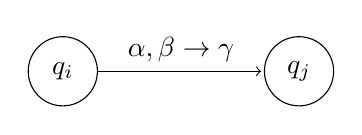
\begin{tikzpicture}[shorten >=1pt,node distance=3cm,on grid,auto]
\node[state] (q_i) {$q_i$};
\node[state] (q_j) [right=of q_i] {$q_j$};
\path[->]
(q_i) edge node {$\alpha,\beta \to \gamma$} (q_j);
\end{tikzpicture} \\
\end{minipage}


\begin{tcolorbox}
\[
\{x^ay^bz^c : a=b\text{ or } a = c \}
\]
\end{tcolorbox}


\paragraph{b)} 
Design a PDA to recognize language $ L=\{x^n y^{m+n} x^m \mid \; n,m \geq 0; \; n,m \in \mathbb{N}  \} $  \hfill \small{(5/30 pts)} \\

\begin{tcolorbox}
\iffalse
Pushdows automata recognize context-free languages. There is a pushdown automata for every context-free language.
Context-free languages are closed under concatenation.
The given language $L$ can be understood as the concatenation of the following two languages:
\[
\{x^ny^n~|~n\geq0;~n\in N\}
\]
\[
\{y^mx^m~|~m\geq0;~m\in N\}
\]
We could say the corresponding grammars are:
\[
    S_1  \rightarrow xS_1y~|~e
\]
and
\[
S_2 \rightarrow yS_2x ~|~ e
\]
The new grammar can be described as
\[
G=(V_1\cup V_2\cup \{S\}, \Sigma_1\cup\Sigma_2, R_1\cup R_2 \cup \{S \rightarrow S_1S_2\}, S)
\]
\begin{align*}
    S & \rightarrow S_1S_2 \\
    S_1 & \rightarrow xS_1y ~ | ~ e\\
    S_2 & \rightarrow yS_2x ~ |~ e
\end{align*}
\fi
\begin{center}
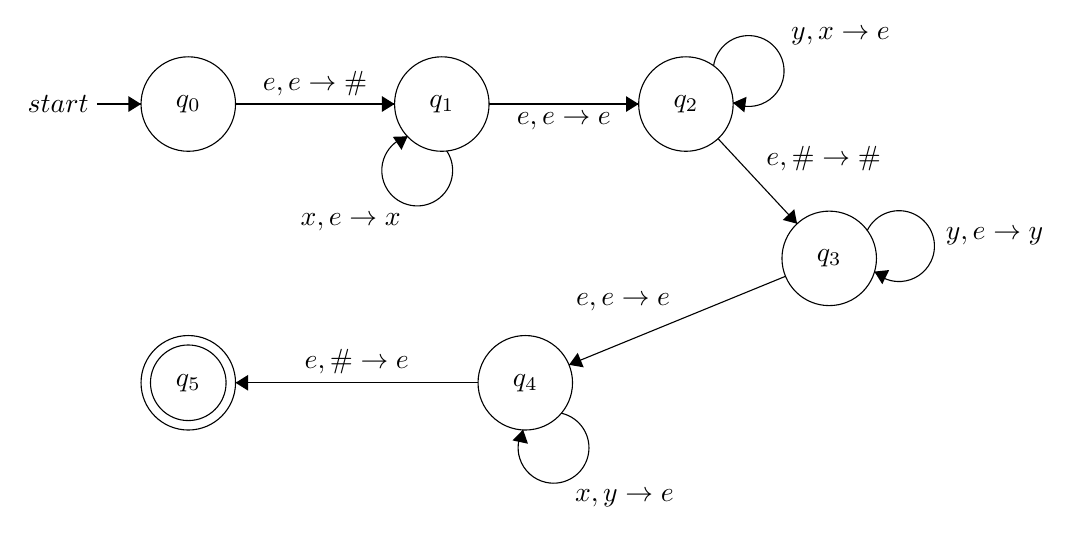
\begin{tikzpicture}[scale=0.2]
\tikzstyle{every node}+=[inner sep=0pt]
\draw [black] (11.9,-5.8) circle (3);
\draw (11.9,-5.8) node {$q_0$};
\draw [black] (28,-5.8) circle (3);
\draw (28,-5.8) node {$q_1$};
\draw [black] (43.5,-5.8) circle (3);
\draw (43.5,-5.8) node {$q_2$};
\draw [black] (52.6,-15.6) circle (3);
\draw (52.6,-15.6) node {$q_3$};
\draw [black] (33.3,-23.5) circle (3);
\draw (33.3,-23.5) node {$q_4$};
\draw [black] (11.9,-23.5) circle (3);
\draw (11.9,-23.5) node {$q_5$};
\draw [black] (11.9,-23.5) circle (2.4);
\draw [black] (14.9,-5.8) -- (25,-5.8);
\fill [black] (25,-5.8) -- (24.2,-5.3) -- (24.2,-6.3);
\draw (19.95,-5.3) node [above] {$e,e\rightarrow \#$};
\draw [black] (6.1,-5.8) -- (8.9,-5.8);
\draw (5.6,-5.8) node [left] {$start$};
\fill [black] (8.9,-5.8) -- (8.1,-5.3) -- (8.1,-6.3);
\draw [black] (31,-5.8) -- (40.5,-5.8);
\fill [black] (40.5,-5.8) -- (39.7,-5.3) -- (39.7,-6.3);
\draw (35.75,-6.3) node [below] {$e,e\rightarrow e$};
\draw [black] (45.54,-8) -- (50.56,-13.4);
\fill [black] (50.56,-13.4) -- (50.38,-12.48) -- (49.65,-13.16);
\draw (48.58,-9.24) node [right] {$e,\#\rightarrow \#$};
\draw [black] (28.309,-8.772) arc (33.67416:-254.32584:2.25);
\draw (22.21,-12.72) node [below] {$x,e\rightarrow x$};
\fill [black] (25.83,-7.85) -- (24.89,-7.88) -- (25.44,-8.71);
\draw [black] (45.255,-3.381) arc (171.76754:-116.23246:2.25);
\draw (50.15,-1.5) node [right] {$y,x\rightarrow e$};
\fill [black] (46.49,-5.72) -- (47.21,-6.33) -- (47.35,-5.34);
\draw [black] (55.011,-13.834) arc (153.95525:-134.04475:2.25);
\draw (59.97,-14.18) node [right] {$y,e\rightarrow y$};
\fill [black] (55.47,-16.44) -- (55.97,-17.24) -- (56.41,-16.34);
\draw [black] (49.82,-16.74) -- (36.08,-22.36);
\fill [black] (36.08,-22.36) -- (37.01,-22.52) -- (36.63,-21.6);
\draw (39.51,-18.99) node [above] {$e,e\rightarrow e$};
\draw [black] (30.3,-23.5) -- (14.9,-23.5);
\fill [black] (14.9,-23.5) -- (15.7,-24) -- (15.7,-23);
\draw (22.6,-23) node [above] {$e,\#\rightarrow e$};
\draw [black] (35.581,-25.43) arc (77.49857:-210.50143:2.25);
\draw (39.59,-30.23) node [below] {$x,y\rightarrow e$};
\fill [black] (33.16,-26.48) -- (32.49,-27.16) -- (33.47,-27.37);
\end{tikzpicture}
\end{center}
\end{tcolorbox}
\newpage

\paragraph{c)} 
Design a PDA to recognize language $ L=\{x^n y^m \mid \; n < m \leq 2n; \; n,m \in \mathbb{N^+} \} $  \hfill \small{(10/30 pts)} \\
Do not use multi-symbol push/pop operations in your transitions. \\
Simulate the PDA on strings \textit{xxy} (with only one rejecting derivation) and \textit{xxyyyy} (accepting derivation) with transition tables. \\


\begin{tcolorbox}
\begin{center}
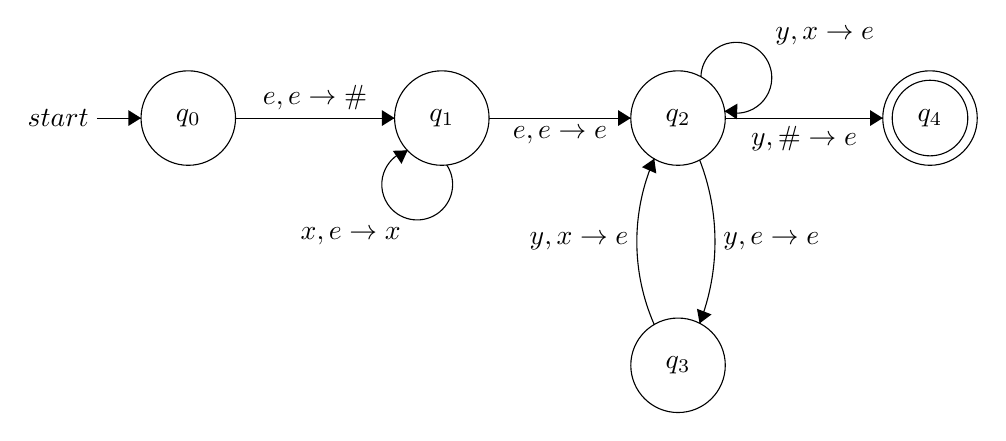
\begin{tikzpicture}[scale=0.2]
\tikzstyle{every node}+=[inner sep=0pt]
\draw [black] (11.9,-5.8) circle (3);
\draw (11.9,-5.8) node {$q_0$};
\draw [black] (28,-5.8) circle (3);
\draw (28,-5.8) node {$q_1$};
\draw [black] (43,-5.8) circle (3);
\draw (43,-5.8) node {$q_2$};
\draw [black] (43,-21.5) circle (3);
\draw (43,-21.5) node {$q_3$};
\draw [black] (59,-5.8) circle (3);
\draw (59,-5.8) node {$q_4$};
\draw [black] (59,-5.8) circle (2.4);
\draw [black] (14.9,-5.8) -- (25,-5.8);
\fill [black] (25,-5.8) -- (24.2,-5.3) -- (24.2,-6.3);
\draw (19.95,-5.3) node [above] {$e,e\rightarrow\#$};
\draw [black] (6.1,-5.8) -- (8.9,-5.8);
\draw (5.6,-5.8) node [left] {$start$};
\fill [black] (8.9,-5.8) -- (8.1,-5.3) -- (8.1,-6.3);
\draw [black] (31,-5.8) -- (40,-5.8);
\fill [black] (40,-5.8) -- (39.2,-5.3) -- (39.2,-6.3);
\draw (35.5,-6.3) node [below] {$e,e\rightarrow e$};
\draw [black] (28.309,-8.772) arc (33.67416:-254.32584:2.25);
\draw (22.21,-12.72) node [below] {$x,e\rightarrow x$};
\fill [black] (25.83,-7.85) -- (24.89,-7.88) -- (25.44,-8.71);
\draw [black] (44.453,-3.189) arc (178.64214:-109.35786:2.25);
\draw (49.15,-0.61) node [right] {$y,x\rightarrow e$};
\fill [black] (45.96,-5.36) -- (46.74,-5.88) -- (46.77,-4.88);
\draw [black] (44.372,-8.462) arc (21.26604:-21.26604:14.305);
\fill [black] (44.37,-18.84) -- (45.13,-18.27) -- (44.2,-17.91);
\draw (45.85,-13.65) node [right] {$y,e\rightarrow e$};
\draw [black] (41.489,-18.916) arc (-156.25947:-203.74053:13.08);
\fill [black] (41.49,-8.38) -- (40.71,-8.92) -- (41.62,-9.32);
\draw (39.88,-13.65) node [left] {$y,x\rightarrow e$};
\draw [black] (46,-5.8) -- (56,-5.8);
\fill [black] (56,-5.8) -- (55.2,-5.3) -- (55.2,-6.3);
\draw (51,-6.3) node [below] {$y,\#\rightarrow e$};
\end{tikzpicture}
\end{center}
\begin{minipage}{0.45\textwidth}
\begin{tabular}{c|c|c}
     State & Unread Input & Stack  \\
     $q_0$& xxy & e\\
     $q_1$&xxy&\#\\
     $q_1$&xy&x\#\\
     $q_1$&y&xx\#\\
     $q_2$&y&xx\#\\
     $q_2$&e&x\#
\end{tabular}
\end{minipage}
    \begin{minipage}{0.45\textwidth}
\begin{tabular}{c|c|c}
     State & Unread Input & Stack  \\
     $q_0$& xxyyyy & e\\
     $q_1$&xxyyyy&\#\\
     $q_1$&xyyyy&x\#\\
     $q_1$&yyyy&xx\#\\
     $q_2$&yyyy&xx\#\\
     $q_3$&yyy&xx\#\\
     $q_2$&yy&x\#\\
     $q_2$&y&\#\\
     $q_4$&e&e
\end{tabular}
\end{minipage}
\end{tcolorbox}

\paragraph{d)} Given two languages $L'$ and $L$ as $L'=\{w \mid \; w\in L; \; |w|=4n+2 \; for\; n\in \mathbb{N} \}$
\hfill \small{(10/30 pts)} \\
If $L$ is a CFL, show that $L'$ is also a CFL by constructing an automaton for $L'$ in terms of another automaton that recognizes $L$. \\


\begin{tcolorbox}
 Using \textit{Cross Product Construction}, we will define a new PDA to recognize the language $|w| = 4n+2$. This language is regular$(\Sigma\Sigma(\Sigma\Sigma\Sigma\Sigma)^*)$ and can be constructed since regular languages are recognized by FSM's. Every transition moves the PDA for L and L'. In the new PDA, the stack is used only by the PDA for L. Moreover, the input string is accepted only when both of the automata landed on accepting states and the stack is empty. To formally define the new PDA, we use:
 \[
 M = (K_1\times K_2, \Sigma, \Gamma, \Delta, (S_1,S_2), F_1\times F_2)
 \]
 Where the $\Delta$ is changed according to the necessary modifications.
 \[
 (((q_1,q_2), a, \beta), ((\delta_1(q_1),\delta_2(q_2)), \gamma))
 \]
 Where $\delta_1$ and $\delta_2$ functions are for transitions for the automata for recognizing L and $|w|=4n+2$, respectively. A more detailed explanation for construction of intersection of PDA and FSM is present in next page, answer for 4.b.
\end{tcolorbox}






\newpage
\section{Closure Properties \hfill \normalfont{(20 pts)}}

Let $L_1$ and $L_2$ be context-free languages which are not regular, and let $L_3$ be a regular language. Determine whether the following languages are necessarily CFLs or not. If they need to be context-free, explain your reasoning. If not, give one example where the language is a CFL and a counter example where the language is not a CFL. \\

\paragraph{a)} $L_4 = L_1 \cap (L_2 \setminus L_3)$ \hfill \small{(10/20 pts)} \\

\begin{tcolorbox}
Let $L_1$ be the language
\[
\{a^nb^mc^k : n=m;~ n,m>0\}
\]
and $L_2$ be the language
\[
\{a^nb^mc^k : m=k;~m,k>0\}
\]
Both languages are context free and not regular.
Let $L_3$ be $\{e\}$ where $e$ is the empty string. Thus making $L_2\setminus L_3 = L_2$. Hence $L_4 = L_1 \cap L_2 = \{a^nb^nc^n \}$. $L_4$ is not context-free.
\end{tcolorbox}

\paragraph{b)} $L_5 = (L_1 \cap L_3)\text{*}$ \hfill \small{(10/20 pts)} \\

\begin{tcolorbox}
The intersection of a context-free language and a regular language is context-free. Thus $L_1\cap L_3$ is context-free. If L is a context free language and R is a regular language, then $L = L(M_1)$ for some pushdown automaton $M_1=(K_1,\Sigma, \Gamma_1, \Delta_1, s_1, F_1)$, and $R = L(M_2)$ for some deterministic finite automaton $M_2=(K_2,\Sigma,\delta,s_2,F_2)$. The idea is to combine these machines into a single pushdown automaton M that carries out computations by $M_1$ and $M_2$ in parallel and accepts only if both would have accepted. Specifically, let $M=(K,\Sigma,\Gamma, \Delta,s,F)$ where
\begin{align*}
    K &= K_1\times K_2\\
s&=(s_1,s_2)\\
F&=F_1\times F_2
\end{align*}
$\Delta$, the transition relation, is defined as follows. For each transition of the pushdown automaton $((q_1,a,\beta),(p_1,\gamma))\in \Delta_1$, and for each state $q_2\in K_2$, we add to $\Delta$ the transition $(((q_1,q_2),a,\beta),((p_1,\delta(q_2,a)),\gamma))$; and for each transition of the form $((q_1,e,\beta),(p_1,\gamma))\in\Delta_1$ and each state $q_2\in K_2$, we add to $\Delta$ the transition $(((q_1,q_2),e,\beta),((p_1,q_2),\gamma))$. That is, M passes from state $(q_1,q_2)$ to state $p_1,p_2$ in the same way that $M_1$ passes from state $q_1$ to $p_1$, except that in addition M keeps track of the change in the state of $M_2$ caused by reading the same input.
Moreover, context-free languages are closed under \textit{Kleene Star}. \textit{Kleene Star} of a context free language $L(G_1)^*$ is generated by
\[
G=(V_1 \cup \{S\}, \Sigma_1, R_1\cup \{S\rightarrow e, S\rightarrow SS_1\},S)
\]
Hence, $L_5$ is context-free.
\end{tcolorbox}





\newpage
\section{Pumping Theorem \hfill \normalfont{(20 pts)}}

\paragraph{a)} Show that $L=\{a^n m^n t^i \mid \; n\leq i \leq 2n\}$ is not a Context Free Language \hfill \small{(10/20 pts)} \\
using Pumping Theorem for CFLs. \\

\begin{tcolorbox}
Let p be the pumping length, choose $w=a^pm^pt^p\in L$. We see that $|w| \geq p$ and there must be some decomposition $w=uxyzv$ such that $|xyz| \leq p$. Then, there are two cases for which the first one is $xyz$ contains a or m, and the second case is $xyz$ consists of only t's. In the former case, the decomposition must happen exactly at the middle of a's and m's such that $x=a^k$, $y=am(\text{or }aamm\text{ or }e)$, $z=m^k$ in order to keep the number of a's and m's the same. Otherwise, the resulting word would not be in L. If we pump from that split, we get a word $w'=a^{p+k}m^{p+k}t^p\notin L$ since $p+k>p$. Thus, there is no way to make the decomposition in this case. Trying the other case, $xyz=t^k$, we could choose arbitrary $a,b,c$ such that $x=t^a$, $y=t^b$, $z=t^c$.  Since $a+c>0$, when we pump it 3p times, we get $w'=a^pm^pt^{3pa+pb+3pc}\notin L$ because $3p(a+c) > 2p$. Thus, there is no way to make a decomposition and L is not context free.
\end{tcolorbox}


\paragraph{b)} Show that $L=\{a^n b^{2n} a^n \mid \; n \in \mathbb{N+} \}$ is not a Context Free Language \hfill \small{(10/20 pts)} \\
using Pumping Theorem for CFLs. \\

\begin{tcolorbox}
Let $p$ be the pumping length, also choose $w=a^pb^{2p}a^p\in L$. We see that $|w| \geq p$. So, there must be some decomposition $w=uxyzv$ such that $ux^iyz^iv\in L$ for all $i \geq 0$. We will show that no such decomposition exists and the language is not context free. We have that $|xyz| \leq p$. So, $xyz$ cannot contain both a's from left and right of b's. When inspecting $w$ case by case, first choose some $xyz$ such that there is no a from right of b's. $xyz$ may include a's from the left of b's and also may not include. If it included, then the equality of the number of a's from the left of b's and the number of a's from the right of b's would be broken. Hence, this word is not in L. If it did not include a's (pumping only b's), then the number of b's would no longer be equal to two times the number of a's from right and left sides. The other case ($xyz$ does not contains a's from left of b's) is symmetric to this one and same reasoning could be applied. Hence, L is not context free.
\end{tcolorbox}





\newpage
\section{CNF and CYK \hfill \normalfont{(not graded)}}

\paragraph{a)} Convert the given context-free grammar to Chomsky Normal Form. \\

$ S   \to XSX \mid xY $ \\
$ X   \to Y \mid S $ \\
$ Y   \to z \mid \varepsilon $ \\

\begin{tcolorbox}
answer here ...
\vspace{18cm} % remove this after your answer
\end{tcolorbox}


\paragraph{b)} Use the grammar below to parse the given sentence using Cocke–Younger–Kasami algorithm. \\
Plot the parse trees. \\

\begin{multicols}{2}
S $\to$ NP VP \\
S $\to$ X1 VP \\
X1 $\to$ Aux NP \\
S $\to$ book $\mid$ include $\mid$ prefer \\
S $\to$ Verb NP \\
S $\to$ X2 PP \\
S $\to$ Verb PP \\
S $\to$ VP PP \\
NP $\to$ I $\mid$ she $\mid$ me $\mid$ Houston \\
NP $\to$ Det Nom \\
Nom $\to$ book $\mid$ flight $\mid$ meal $\mid$ money \\
Nom $\to$ Nom Noun \\
Nom $\to$ Nom PP \\
VP $\to$ book $\mid$ include $\mid$ prefer \\
VP $\to$ Verb NP \\
VP $\to$ X2 PP \\
X2 $\to$ Verb NP \\
VP $\to$ Verb PP \\
VP $\to$ VP PP \\
PP $\to$ Prep NP \\
Det $\to$ that $\mid$ this $\mid$ the $\mid$ a \\
Noun $\to$ book $\mid$ flight $\mid$ meal $\mid$ money \\
Verb $\to$ book $\mid$ include $\mid$ prefer \\
Aux $\to$ does \\
Prep $\to$ from $\mid$ to $\mid$ on $\mid$ near $\mid$ through \\
\end{multicols}

\vspace{5mm}

book the flight through Houston \\

\begin{tcolorbox}

\scriptsize

Empty parse table:\\
\begin{tikzpicture}[node distance=0cm, outer sep = 0pt]

\node[terminal] (l0) {
    \begin{tabular}{@{}P{2.9cm}|@{}P{2.9cm}|@{}P{2.9cm}|@{}P{2.9cm}|@{}P{2.9cm}}
    book & the & flight & through & Houston \\
    \end{tabular}
};

\node[nonterminal] (l1) [above = of l0] {
    \begin{tabular}{@{}P{2.9cm}|@{}P{2.9cm}|@{}P{2.9cm}|@{}P{2.9cm}|@{}P{2.9cm}}
    1:1 & 
    2:2 & 
    3:3 & 
    4:4 & 
    5:5 \\
    \end{tabular}
};

\node[nonterminal] (l2) [above = of l1.north] {
    \begin{tabular}{@{}P{2.9cm}|@{}P{2.9cm}|@{}P{2.9cm}|@{}P{2.9cm}}
    1:2 $\to$ 1:1 2:2 & 
    2:3 $\to$ 2:2 3:3 & 
    3:4 $\to$ 3:3 4:4 & 
    4:5 $\to$ 4:4 5:5 \\
    \end{tabular}
};

\node[nonterminal] (l3) [above = of l2.north] {
    \begin{tabular}{@{}P{2.9cm}|@{}P{2.9cm}|@{}P{2.9cm}}
        \begin{tabular}{@{}l} 1:3 $\to$ 1:1 2:3 \\ 1:3 $\to$ 1:2 3:3 \end{tabular}& 
        \begin{tabular}{@{}l} 2:4 $\to$ 2:2 3:4 \\ 2:4 $\to$ 2:3 4:4 \end{tabular}& 
        \begin{tabular}{@{}l} 3:5 $\to$ 3:3 4:5 \\ 3:5 $\to$ 3:4 5:5 \end{tabular}\\
    \end{tabular}
};

\node[nonterminal] (l4) [above = of l3.north] {
    \begin{tabular}{@{}P{2.9cm}|@{}P{2.9cm}}
        \begin{tabular}{@{}l}1:4 $\to$ 1:1 2:4 \\ 1:4 $\to$ 1:2 3:4 \\ 1:4 $\to$ 1:3 4:4 \end{tabular}& 
        \begin{tabular}{@{}l}2:5 $\to$ 2:2 3:5 \\ 2:5 $\to$ 2:3 4:5 \\ 2:5 $\to$ 2:4 5:5 \end{tabular}\\
    \end{tabular}
};

\node[nonterminal] (l5) [above = of l4.north] {
    \begin{tabular}{@{}P{2.9cm}}
        \begin{tabular}{@{}l}
        1:5 $\to$ 1:1 2:5 \\ 1:5 $\to$ 1:2 3:5 \\ 
        1:5 $\to$ 1:3 4:5 \\ 1:5 $\to$ 1:4 5:5 
        \end{tabular}\\
    \end{tabular}
};

\end{tikzpicture}\\\\

rest of the answer here ...\\
\vspace{4cm} % remove this after your answer
\end{tcolorbox}



\newpage
\section{Deterministic Pushdown Automata \hfill \normalfont{(not graded)}}
Provide a DPDA to recognize the given languages, the DPDA must read its entire input and finish with an empty stack.
\paragraph{a)} $a^*bc \cup a^nb^nc$ \\

\begin{tcolorbox}
answer here ...
\vspace{12cm} % remove this after your answer
\end{tcolorbox}

\newpage

\paragraph{b)} $(aa)^*c \cup a^nb^nc$ \\

\begin{tcolorbox}
answer here ...
\vspace{12cm} % remove this after your answer
\end{tcolorbox}



\end{document}